\documentclass{ltjarticle}

\usepackage{graphicx}
\usepackage{hyperref}
\usepackage{subcaption}
\usepackage{xcolor}
\usepackage{amssymb}
\usepackage{amsmath}

\usepackage[backend=biber,style=numeric]{biblatex}
\addbibresource{references.bib}

\title{Identifying Woodblocks from the Bukan Collection}
\author{Thomas Leyh}
\date{March 20th, 2020}

\begin{document}

\maketitle

\section{Introduction}

The \emph{Center for Open Data in the Humanities} (CODH) is a joint research institution in Tokyo, Japan. Its goal is the promotion of data-driven research in the humanities.\cite{kitamoto2017codh} For this purpose they were releasing a number of data sets, all of them related to Japanese history and arts. This work started out by specifically looking at the \emph{Bukan Collection}\cite{codh2018bukan}, around 370 books with information about government officials during the 18th and 19th century. So, how can we assist humanities researchers with techniques from Computer Science?

By applying well-known algorithms from Computer Vision on the books' pages, without using information about the written content, we were able to develop a reliable system for spotting and visualizing similarities. This might be a first step into building a timeline of a book's prints, thus exposing some historical events hidden in there.

But more importantly, this is an example of how even conservative algorithms can give compelling results by using a few reasonable assumptions on the corresponding data. Even basic computer-aided quantitative analysis might reveal information that is near invisible to a human researcher.

The full source code of this work can be found at: \url{https://github.com/leyhline/bukan-collection/}

\subsection{The Bukan Collection}

This work was mainly concerned with extracting information from a specific type of book: 武鑑---Bukan. These are historic Japanese books from Edo period (1603-1868). They are about listing people of influence, i.e. persons, families and institutions with governmental responsibilities. Alongside names, there are also various symbols like family crests and procession items as well as family trees. The books are written in pre-modern Japanese (\emph{Kuzushiji}), therefore they can not easily be read without special training. See figure~\ref{fig:shuugyokubukan006} for an example.

\begin{figure}
    \centering
    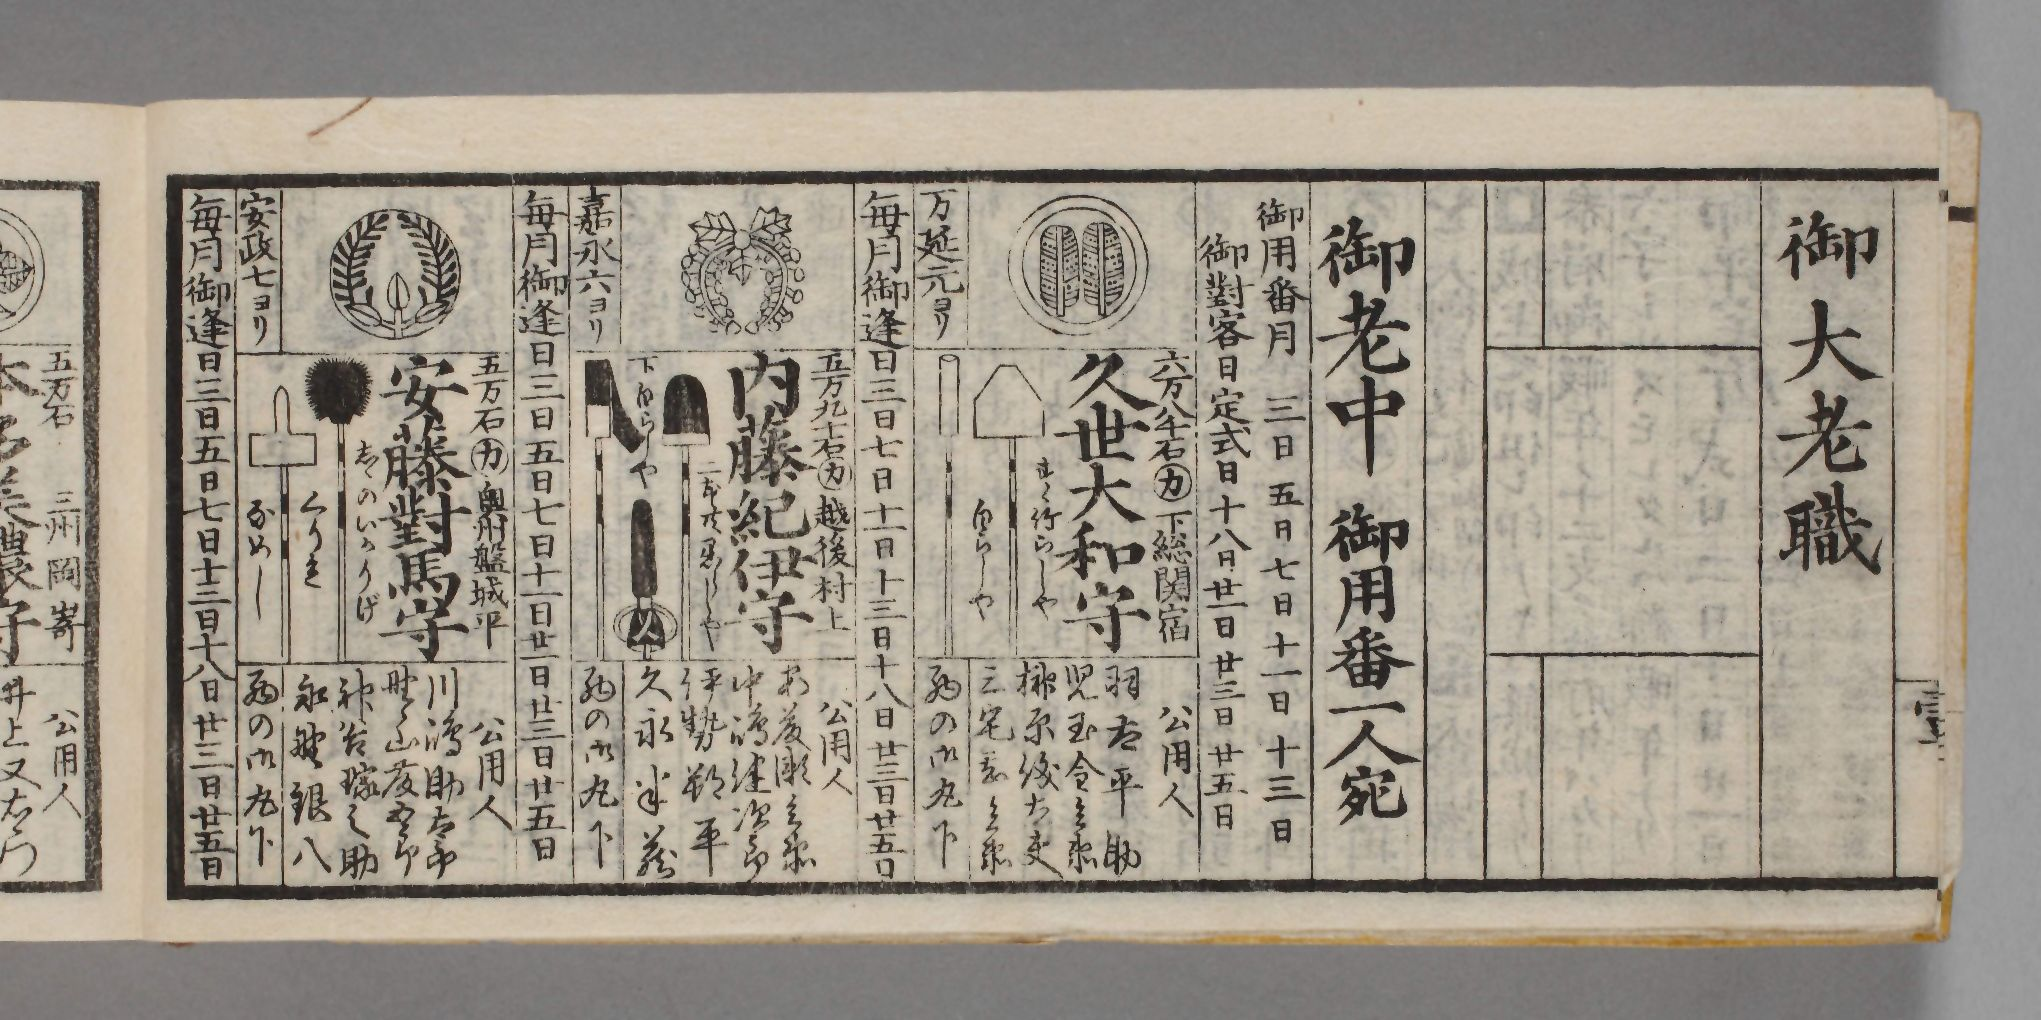
\includegraphics[width=\textwidth]{200019500_00006.jpg}
    \caption[Shūgyoku Bukan (袖玉武鑑), page 6]{Shūgyoku Bukan (袖玉武鑑) from 1861, page 6; showing names, descriptions, family crests and procession items. Especially interesting are the blank areas on the right. These might be filled in later prints.}
    \label{fig:shuugyokubukan006}
\end{figure}

Back then, the Bukan were bestsellers. Often, it was vital knowledge to be able to identify feudal lords and their subordinates. Mistakes when determining the difference in status could easily lead to dispute, sometimes even in a violent manner.\cite{dower1990elements} Nevertheless, publishing of the Bukan was not centralized and therefore not standardized. Especially the layout of the pages---even of books from the same year---might differ to some degree.

The language barrier and the layout difference might seem to complicate the application of common algorithms from Natural Language Processing and Computer Vision. But utilizing the knowledge about the specific data at hand, about the Bukan and especially about their production, we define a problem that is more approachable. This can be done by looking at the printing process.

The books were created using Japanese woodblock-printing. Specialized craftspeople were carving out whole pages from wood. By applying ink on these blocks, numerous prints could be created with comparatively low costs per unit. But it is not like all pages made with the same woodblock would look identical. On the one hand, there are differences in quality of the printed page, stemming from e.g. the amount of ink or the state of the woodblock. On the other hand, the woodblocks itself might have been modified between prints. Some names could have been added, some removed or some symbols modified.

These differences can indicate historical occurrences. Changing family structures like births and deaths as well as gain or loss of status. A scholar in history and old literature will be able to interpret these findings. This work is about supplying her with interactive tools for quickly spotting such sections of interest.

\section{Method}

For tackling this task, three common techniques are used:

\begin{enumerate}
    \item \emph{Keypoint Detection and Matching}, a method from Computer Vision used for finding the same object in different images.
    \item \emph{Projective Transformation} for comparing two different images, regardless their original orientation.
    \item \emph{Relational Databases} for easily storing results as well as querying for relevant pages.
\end{enumerate}

At the end there will be a database populated with the necessary data for easily browsing books, finding similar pages and quickly displaying visualizations. For all these steps free and open tools are available. Especially for the Computer Vision parts the mature \emph{OpenCV} software library was used.\cite{opencv_library}

\subsection{Keypoint Matching}
\label{sec:keypoint-matching}

As a first step, it is necessary to compare a large number of images. This must be computationally viable and invariable to a number of transformations. The original images---as they were stored by the digital camera---have a width of $5616$ and height of $3744$ pixels. Thus, each image has around 21 million pixels with three color chanels each.

\begin{figure}
    \centering
    \begin{subfigure}{.49\textwidth}
        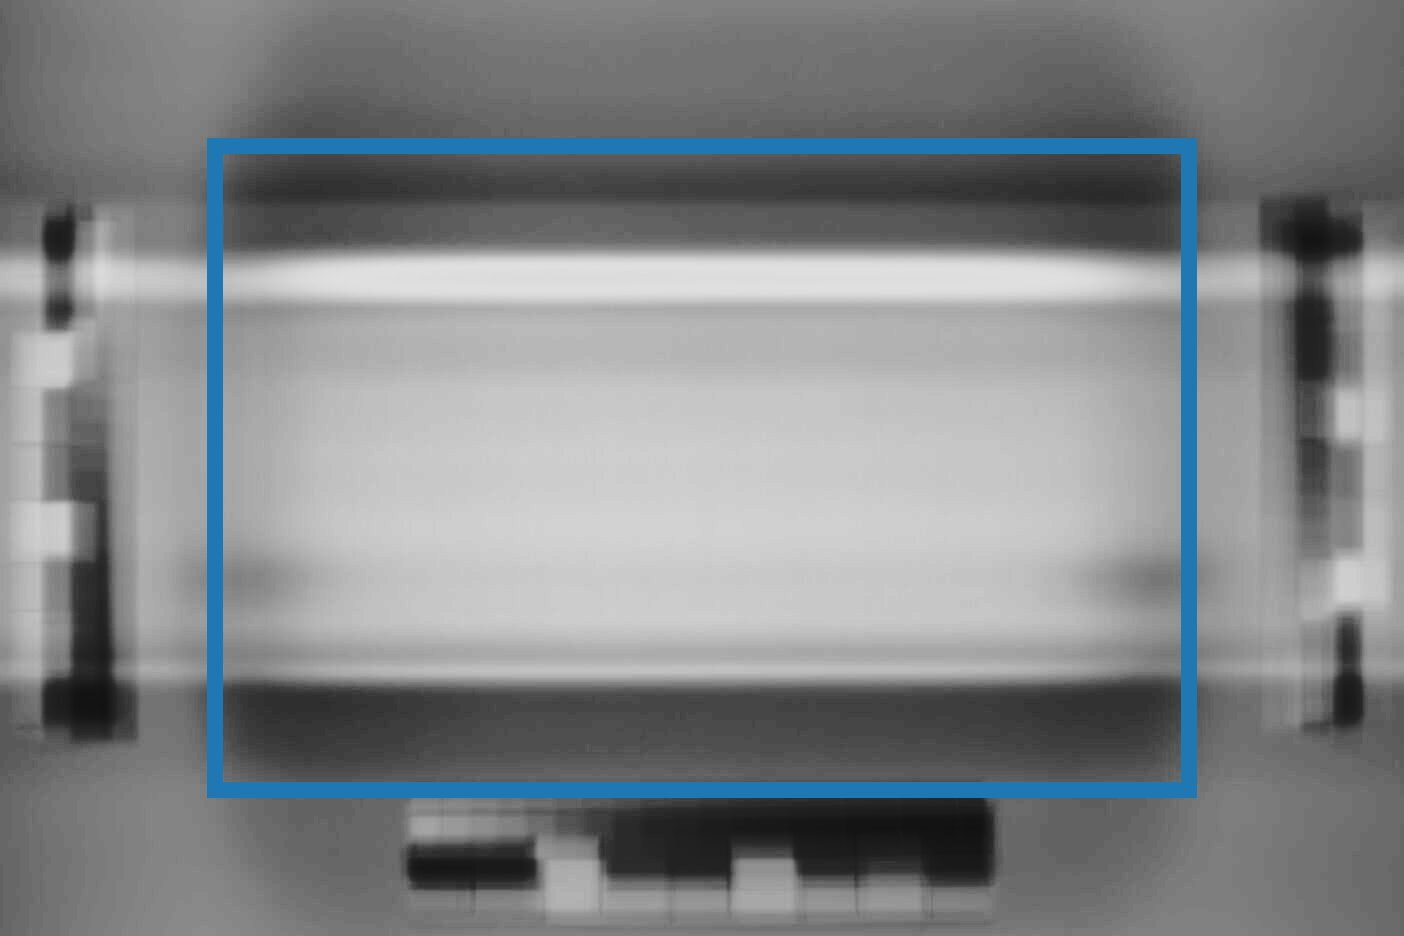
\includegraphics[width=\textwidth]{landscape-average.jpg}
        \caption{}
    \end{subfigure}
    \begin{subfigure}{.49\textwidth}
        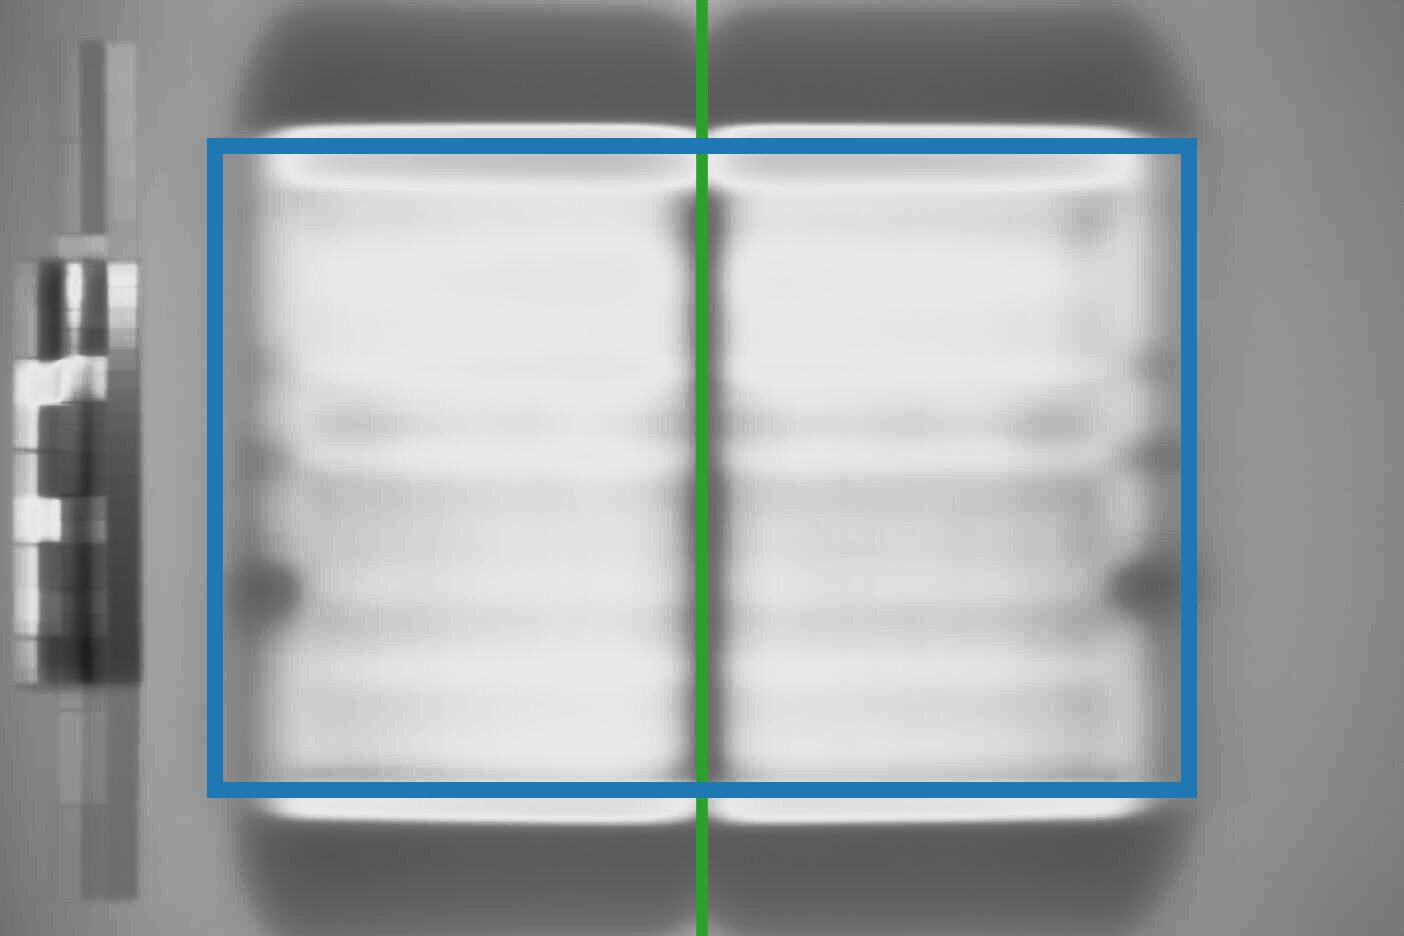
\includegraphics[width=\textwidth]{portrait-average.jpg}
        \caption{}
    \end{subfigure}
    \caption{The mean over all greyscaled images grouped by book layout: (a) shows the mean of scans with wide, single pages while (b) shows images with two pages per scan. The \textcolor{blue}{blue rectangle} shows the cropping window and the \textcolor{olive}{green line} represents the horizontal center of the scan. It seems to correspond with the binding, therefore averagely separating left from right page.}
    \label{fig:average}
\end{figure}

Under the assumption, that this task (1) does not require this level of detail, (2) does not require information about color and (3) only compares the actual pages, not the surrounding area, basic image transformations are applied. All scans are resized by $25\%$, converted to greyscale and finally cropped, resulting in an image shape of $990 \times 660$ pixels. If there are two book pages per scan, they were additionally split at their horizontal center. See figure \ref{fig:average}.

Now, each image has still around $650,000$ pixels. Moreover, at least some \emph{translational invariance} is required since the images are not always perfectly aligned to each other. It is also necessary to consider that letters and symbols vary in thickness, depending on the amount of ink used during printing. This is where \emph{Keypoint Detection} comes in. The general idea is to find points of interest in an image that are most noticable and give an unique description of the local area surrounding them.This description is mostly abstract, hence invariant to many kinds of transformations. For details, see \cite[Ch.4]{szeliski2010computer}

Computer Vision research yielded various kinds of keypoints, most prominently \emph{SIFT}.\cite{lowe2004sift} For evaluating the performance of these algorithms, 12 prints of the \emph{Shūchin Bukan} (袖珍武鑑) were manually annotated, in total around 1800 pages, holding information about the position of matching pages. However, most of the time an identical page number corresponds to matching page content (e.g. page 10 of two prints was made using the same woodblock). To remove this bias, a potential matching of all possible page-keypoint combinations was computed while discarding matching pages where the number of matching keypoints was below a given threshold. The final metric was the intersection of the precision and the recall curve. The following algorithms were evaluated:

\begin{itemize}
    \setlength\itemsep{0em}
    \item ORB\cite{rublee2011orb}
    \item AKAZE\cite{alcantarilla2011fast}
    \item AKAZE without rotational invariance (UPRIGHT)
    \item BRISK\cite{leutenegger2011brisk}
    \item SIFT and SURF\cite{bay2006surf}, but these are not further considered since they are lacking performance on this task
\end{itemize}

\begin{figure}
    \centering
    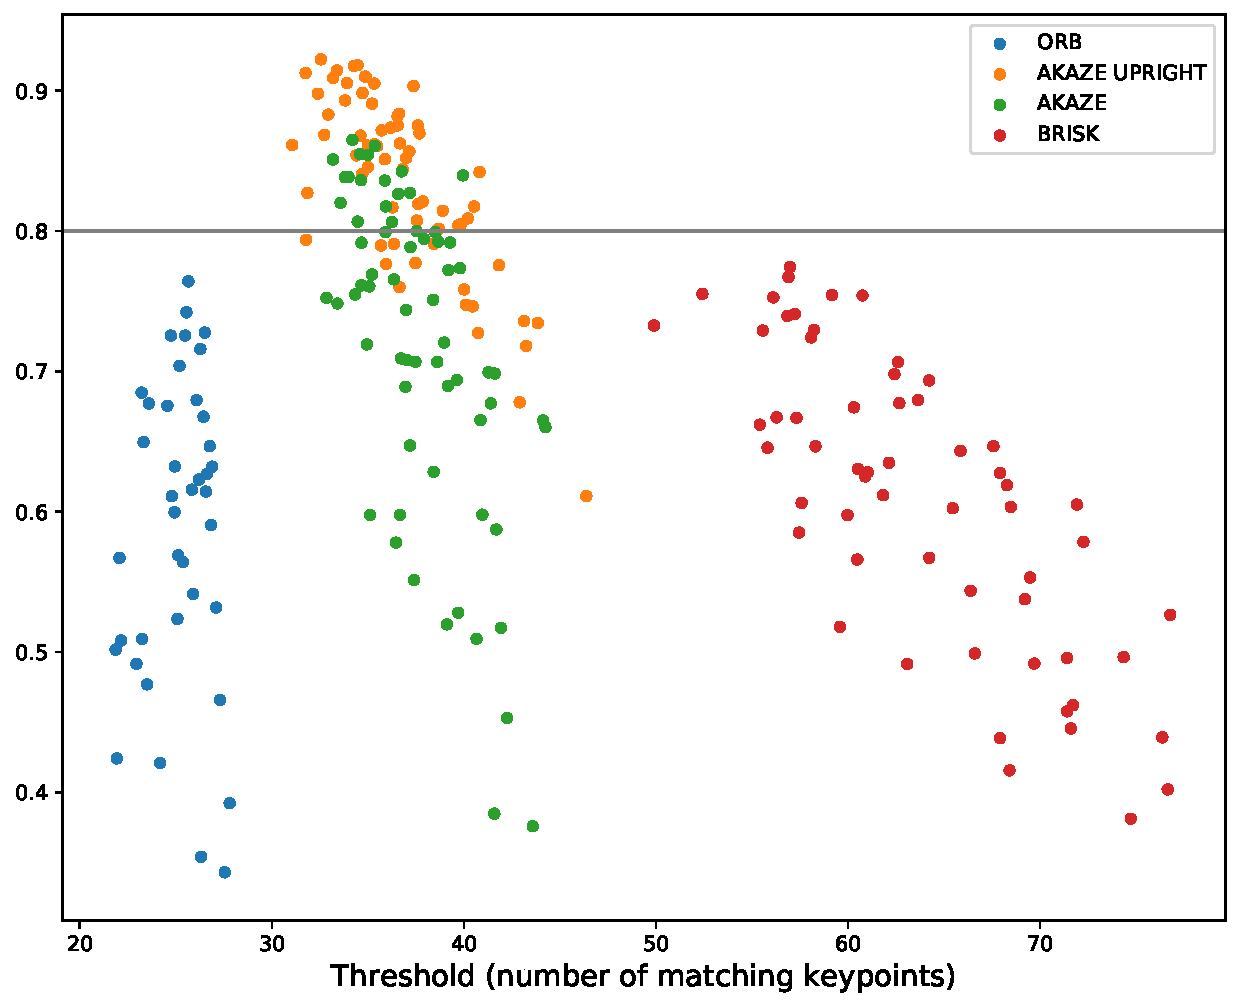
\includegraphics[width=\textwidth]{keypoint-evaluation.pdf}
    \caption{Scatterplot showing the positions of intersection of various precision-recall curves depending on the threshold of the number of matching keypoints. All points above the grey horizontal line at $0.8$ are considered “good enough” by the author. Even though this metric discards much information, there is a general tendency in favor of AKAZE UPRIGHT discernible.}
    \label{fig:keypoint-evaluation}
\end{figure}

The results are presented in figure \ref{fig:keypoint-evaluation}. AKAZE UPRIGHT seems to have the best performance. Here, rotational invariance was explicitly \emph{not} included since the original images were scanned after cleanly aligning them on a table. This seems to bolster the keypoints' discriminative power. Nevertheless, the current results are far from satisfactory; from a performance standpoint as well as from the stability of the approach. Can we improve upon this by incorporating additional information?

\subsection{Projective Transformation}

\begin{figure}
    \centering
    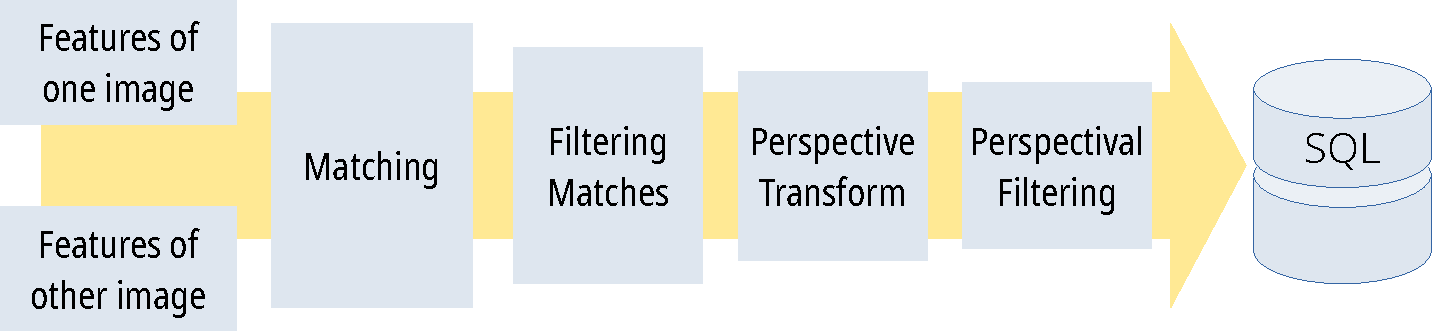
\includegraphics[width=\textwidth]{pipeline.pdf}
    \caption{Starting out from Keypoint Matching described in section~\ref{sec:keypoint-matching} a pipeline was built, reducing the number of false positives by incorporating additional information and storing the results for further usage in a relational database (SQL).}
    \label{fig:pipeline}
\end{figure}

There is, of course, more information that can be used for improving the performance. As a first step, filtering matching keypoints by their quality and position is useful. Here, matches with a distance\footnote{AKAZE keypoints yield binary descriptors. Two such descriptors can be compared calculating the \emph{Hamming Distance}, where a larger distance implies a larger perceptible difference.} over 100 are removed. The same goes for matches, where the keypoint pair is more than 100 pixels apart from each other. With this, larger translations are not allowed since we assume clean alignment during the scanning proces. But by far the largest improvements in performance are gained by attempting a Perspective Transformation between two images.

A Perspective Transformation (or \emph{Homography}) is a matrix $\mathbf{H}$ for transforming homogeneous coordinates $\mathbf{H}\vec{x} = \vec{y}$. This allows for not only linear transformations like translation and rotation but also for perspective transformations. Here, since it is about flat images, the matrix is three-dimensional: $\mathbf{H} \in \mathbb{R}^{3 \times 3}$. Details can be found in most books on Computer Graphics like \cite{marschner2015fundamentals} since these calculations are elementary to modern 3D applications. For finding such a transformation from matching keypoints---even though it is not sure if these matches are always correct---the heuristic \emph{Random Sample Consensus} (RANSAC) algorithm is used.\cite{fischler1981random} Its basic idea is that a random subset of matching keypoint pairs is chosen, using this to compute a transformation and calculating an error metric. By iteratively using different random subsets, eventually the transformation with the smallest error is picked. 

\begin{figure}
    \centering
    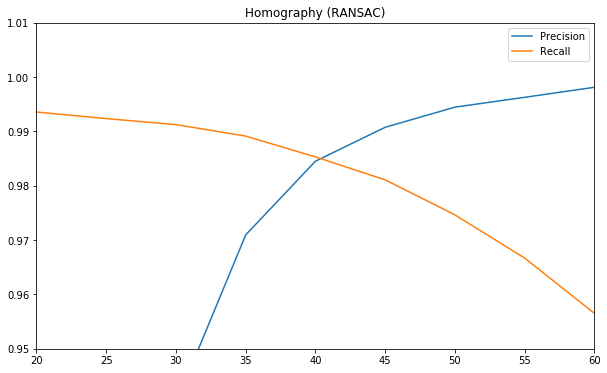
\includegraphics[width=\linewidth]{ransac-performance.png}
    \caption{Precision and recall, by threshold on the number of keypoints. This is but a small part from the whole curve, just showing values above $0.95$. The recall is always on an excellent level while the threshold should not be too low because precision will collapse otherwise.}
    \label{fig:ransac}
\end{figure}

Using RANSAC leads to outstanding results. Values for precision and recall---depending on the threshold set for the number of keypoints---are close to their maximum of $1.0$. Moreover, the performance is much more robust concerning this threshold. See figure~\ref{fig:ransac} where even for larger thresholds the recall is always above $0.95$. These results come at a cost: a computational one. Calculating RANSAC is much more expensive in this regard than just matching keypoints. Of course, first filtering the keypoints before running RANSAC is an option for speeding up the computation, but too aggressive filtering will go at the expense of robustness. After some experiments, a maximum distiance between keypoints of $100$ was chosen.

\begin{figure}
    \centering
    \begin{subfigure}{.49\textwidth}
        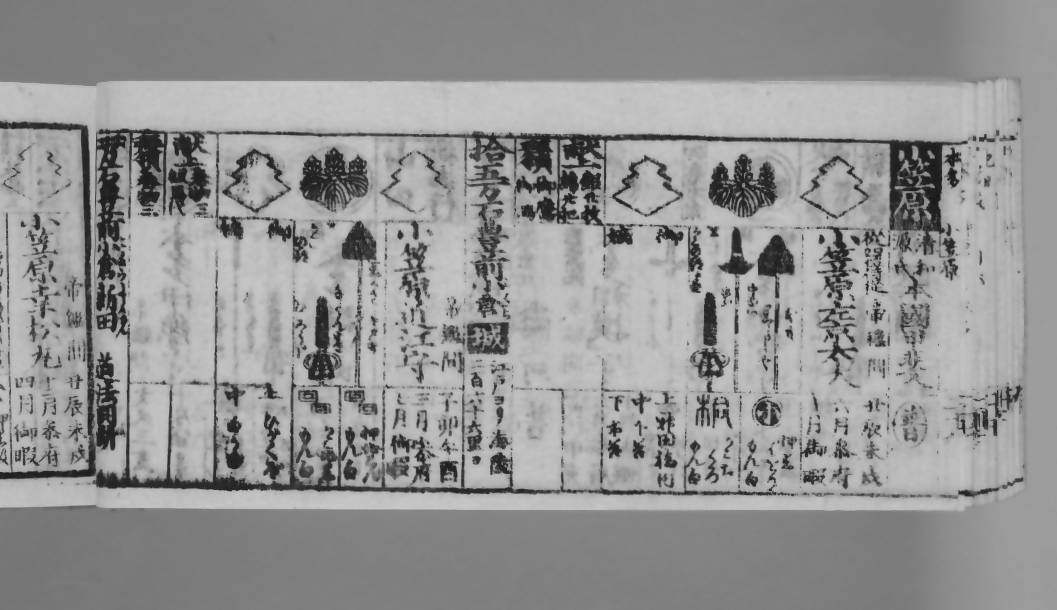
\includegraphics[width=\textwidth]{homography-good.jpg}
        \caption{}
    \end{subfigure}
    \begin{subfigure}{.49\textwidth}
        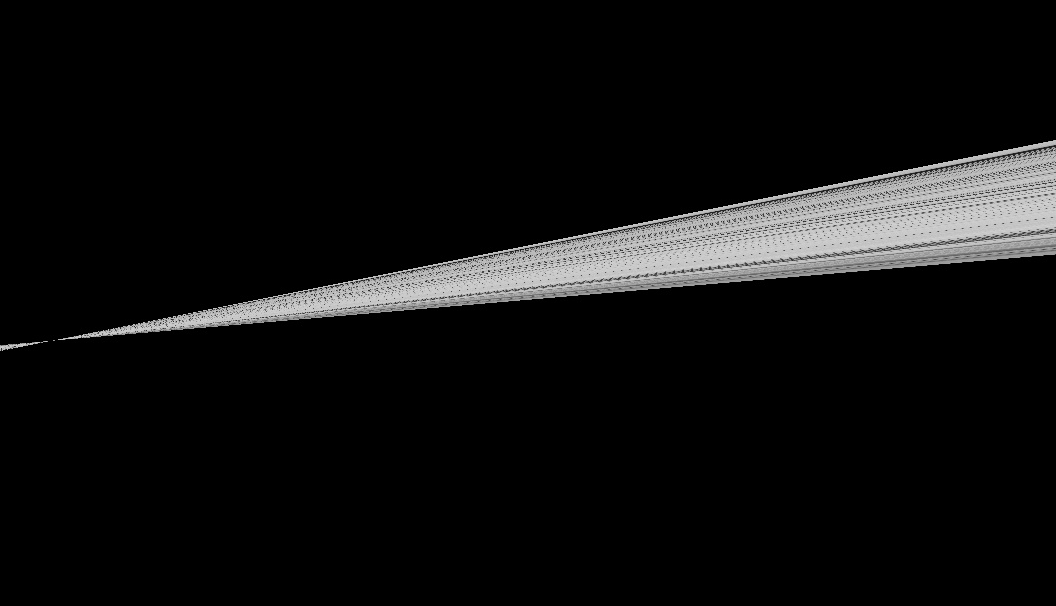
\includegraphics[width=\textwidth]{homography-bad.png}
        \caption{}
    \end{subfigure}
    \begin{subfigure}{\textwidth}
        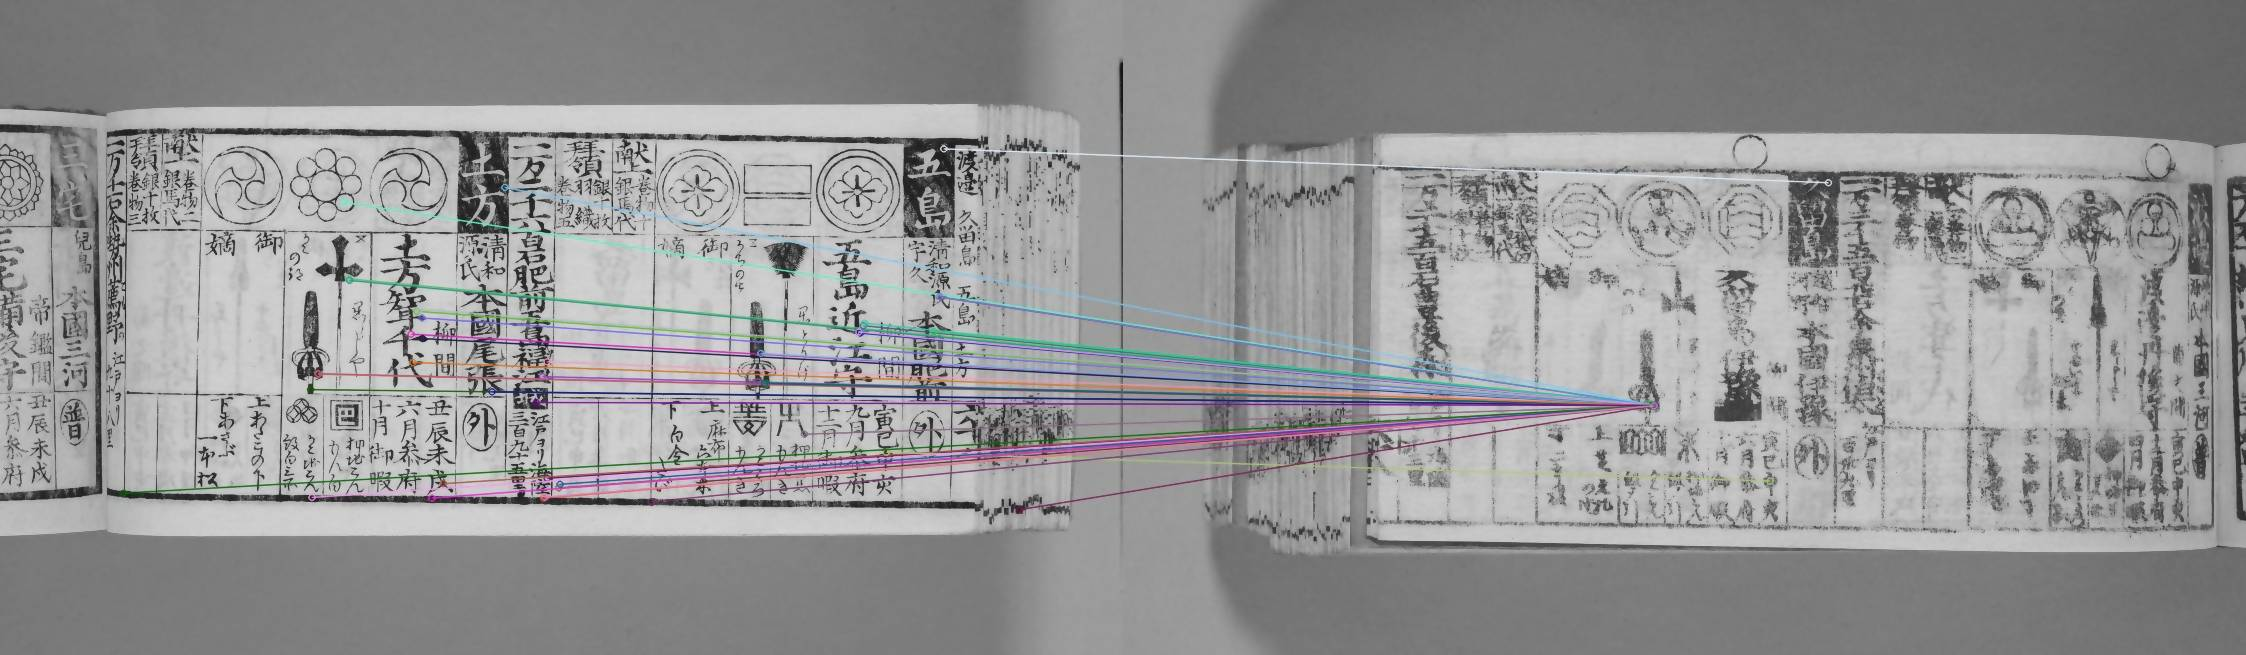
\includegraphics[width=\textwidth]{homography-cause.jpg}
        \caption{}
    \end{subfigure}
    \caption{Two examples for perspective transformations: In this case, a good transformation as in (a) will have no perceptible effect, just slightly shifting some pixels. The image in (b) is the result of a bad transformation, shifting perspective in a way the original image can not be recognized anymore. This is caused by incorrect keypoint matching as seen in (c) where the majority of keypoints on the left page is matched to a single point on the right page.}
    \label{fig:homography-compare}
\end{figure}

A last source of failure that can easily be eliminated are extreme perspective transformations as seen in figure~\ref{fig:homography-compare}. Caused by incorrect keypoint matching, RANSAC mistakenly results in extreme perspective shifts that nevertheless are deemed possible by the algorithm. This makes up for less than $1\%$ of false positives, but can be corrected by removing matches where the projective elements from $\mathbf{H}$ are too extreme. Accordingly, transformations must conform to these two inequalities:

\begin{gather*}
    |\mathbf{H}_{1,3}| \leq 0.001\\
    |\mathbf{H}_{2,3}| \leq 0.001
\end{gather*}

The threshold of $0.001$ is quite conservative and might even be chosen one magnitude lower without much difference.

\subsection{Relational Databases}



\section{Conclusion}

\section{Further Improvements}

\printbibliography

\end{document}
